\capitulo{3}{Conceptos teóricos} \label{cap:conceptos}
Para comprender todo el ecosistema que envuelve a un videojuego, han de ser explicados los distintos términos con los que el proyecto ha tomado contacto y con aquellos en los que se profundizará más adelante.

En este apartado se detallan los conceptos principales y cómo influyen en el desarrollo del juego.

\section{Motor de videojuegos}

El corazón de un videojuego es el motor. Como definición, se trata de una serie de rutinas de programación que forman el núcleo de un juego, permitiendo el diseño, la creación y el funcionamiento de éste. Así mismo, se llama motor de videojuegos al software que permite crearlos \cite{hardz:motgraf}.

Los videojuegos, en su desarrollo, requieren de un entorno que permita englobar todas las herramientas necesarias para poder crearlos. Los motores son el ecosistema perfecto, pues proporcionan herramientas de desarrollo visual y componentes \textit{software} que se pueden reutilizar. Esto es, no es necesario crear desde cero un sistema de físicas, sonido, interacción entre objetos, efectos y otros, sino que todos esos elementos ya los contiene el mismo programa, pudiendo hacer uso de ellos a necesidad del usuario. 

Todo ello conforma el esqueleto del juego, ayudando a los diseñadores, programadores y demás participantes en el proyecto a centrarse en las tareas que han de realizar.

Hay numerosos motores gráficos disponibles al público, donde pueden ser de pago o gratuitos \cite{vand:mejmotgraf}. Actualmente, los tres más potentes en el mercado son gratuitos, donde puede hacerse un uso académico, personal o comercial de ellos (en este último caso hay un límite de ingresos, donde a partir de determinada cifra se empieza a pagar un porcentaje a la compañía para rentabilizar el producto).

En este proyecto se hace uso del motor gráfico Unity.

\subsection{Escena}

Las escenas son el principal elemento fundamental de Unity, motor del que se hablará en el capítulo 4, 'Técnicas y herramientas'. Contienen todos los objetos que componen un nivel, como puede ser todo lo que conforma a los menús, a niveles individuales y cualquier otra cosa. Cada fichero de escena se considera como un marco único \cite{doc:scene}.

\begin{figure}[h]
	\centering
	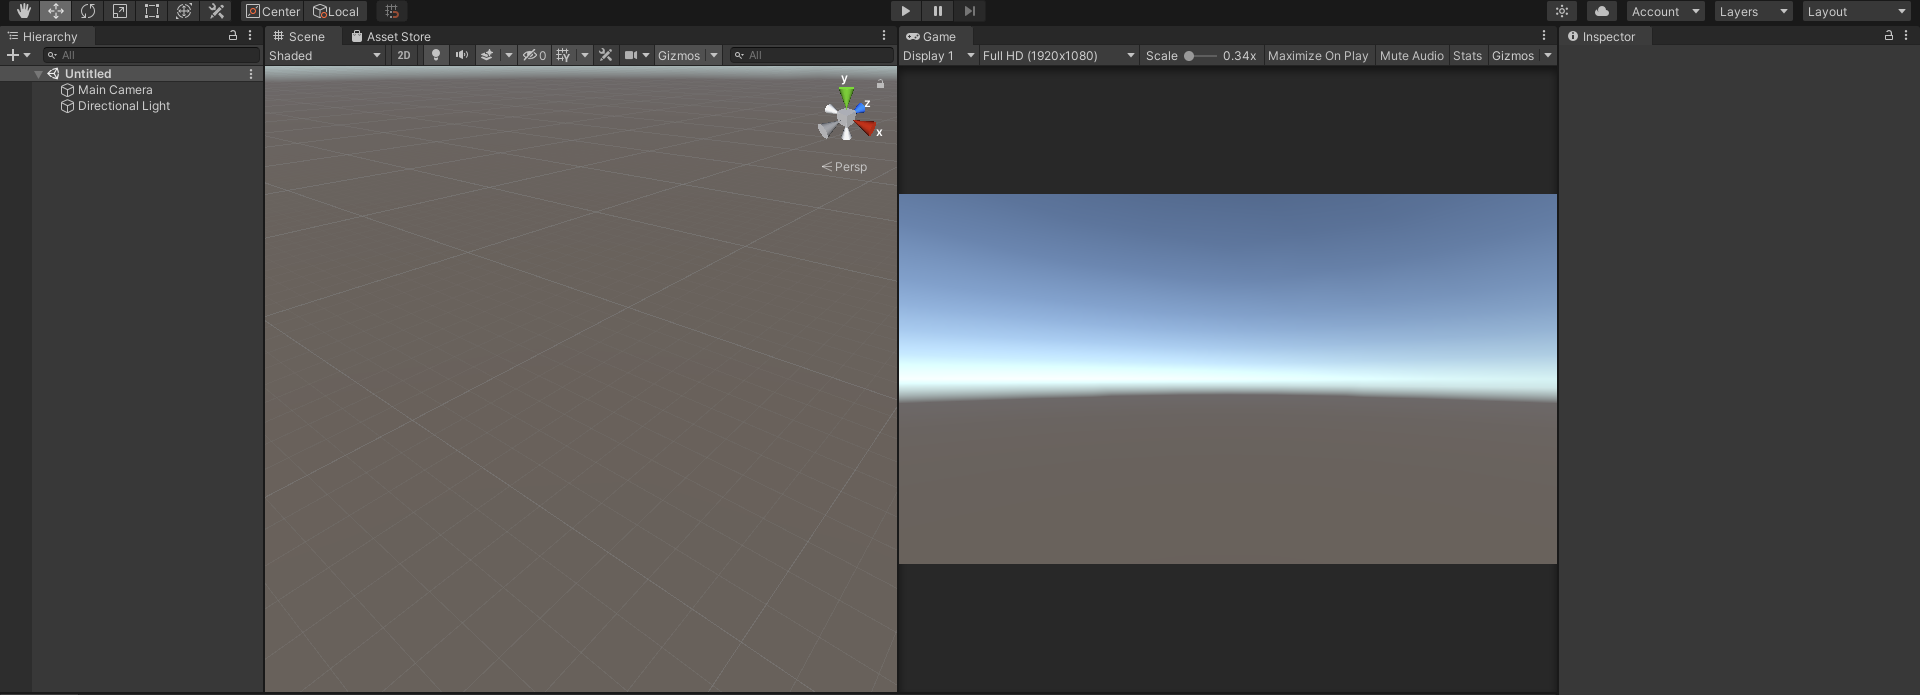
\includegraphics[width=\textwidth]{unity-basic}
	\caption{Escena vacía en el motor de videojuegos Unity.}
	\label{fig:unity-basic}
\end{figure}

\subsection{GameObject}

Se trata de la unidad más básica dentro de una escena. Representa personajes, \textit{props} o elementos de atrezo, y el escenario. Son objetos inertes, sin ninguna funcionalidad de base, por lo que no logran nada por sí mismos, pero sí funcionan como contenedores para componentes, los cuales son los que implementan las funcionalidades a los mismos, como puede ser el movimiento, conteo de vueltas o el sistema de puntos de control entre otros dentro de este proyecto \cite{doc:gameobject}.

Todos los \textit{GameObject} tienen un componente \textit{Transform} o transformada del objeto, que sirve para representar la posición, orientación y escala del objeto respecto al objeto padre del mismo, y en caso de no tener objeto padre será respecto a la escena \cite{doc:transform}. Es uno de los elementos necesarios para poder mover libremente el objeto por el escenario, así como cambiar su tamaño y orientarlo en la posición en la que lo quiera el usuario. La posición del \textit{GameObject} es de tipo \textit{Vector3} y la orientación es de tipo \textit{Quaternion} (en este caso se hace uso de una función llamada ``\textit{Euler}'', siendo los ángulos de \textit{Euler} una representación de una rotación alternativa a los cuaternios expresada como una secuencia de rotaciones entre los ejes cartesianos, primero rotando en Z, luego en X y luego en Y, para devolverla en un vector de tres posiciones).

\begin{figure}[h]
	\centering
	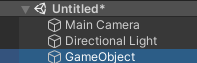
\includegraphics[width=\textwidth]{gameobject}
	\caption{\textit{GameObject} básico ubicado en la jerarquía de objetos.}
	\label{fig:gameobject}
\end{figure}

\subsection{Componentes}

Los componentes son las distintas piezas requeridas para dotar a los objetos de la capacidad de ejercer determinadas acciones o características, como pueden ser las cámaras, el movimiento, el sonido, la luz, las colisiones, los sistemas de conteo y todo lo que aporte Unity por defecto o quiera crear el usuario \cite{doc:component}.

\begin{figure}[h]
	\centering
	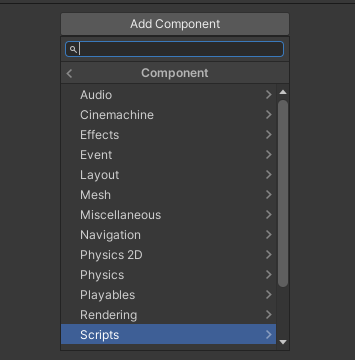
\includegraphics[width=\textwidth]{component-add}
	\caption{Se pueden tanto añadir componentes provistos por Unity como crearlos.}
	\label{fig:component-add}
\end{figure}

Se crean como \textit{scripts} programados en C\#. Estos \textit{scripts} se adjuntan a los \textit{GameObjects}, dando la funcionalidad correspondiente a los objetos en los que se hallen. Gracias a \textit{UnityEngine}, se tienen todas las herramientas para poder programar \textit{scripts} interactuando con los distintos \textit{GameObjects} y el entorno de Unity. No obstante, algunas veces puede ser limitante a la hora de querer modificar alguna característica a bajo nivel, ya que Unity tiene sus propias restricciones a las que el usuario tiene que adaptarse \cite{doc:scripts}.

\begin{figure}[h]
	\centering
	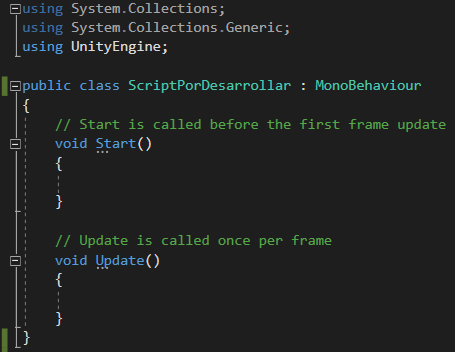
\includegraphics[width=\textwidth]{componente-script}
	\caption{Los \textit{scripts} se programan en C\#.}
	\label{fig:componente-script}
\end{figure}

Los componentes les otorgarán comportamientos específicos, donde los más destacables para este proyecto suministrados por defecto por Unity han sido: 
\begin{itemize}
\tightlist
    \item \textit{Mesh Renderers} o renderizadores de mallas: definen la geometría de los objetos obtenida del \textit{Mesh Filter} (el cual es el encargado de coger una malla de los \textit{assets} y pasárselo al renderizador de malla) y la renderiza en la posición definida por el componente de transformada del objeto para mostrarla en pantalla \cite{doc:meshrenderers}.
    \item \textit{Colliders} o colisionadores: definen la forma de un objeto con el propósito de ejercer colisiones físicas. Este componente es invisible, y no necesariamente tiene la forma exacta que la malla del objeto en cuestión (de hecho, por lo general, una aproximación a menudo es más eficiente para el rendimiento y prácticamente indistinguible en el juego) \cite{doc:colliders}.
   	\begin{itemize}
   	\tightlist
   		    \item \textit{Mesh Colliders} o colisionadores de malla: toma la forma de una malla y construye el colisionador basado en ella. Pueden chocar con otros colisionadores de malla si están marcados como ``convexos'' \cite{doc:meshcolliders}.
   		    \item \textit{Wheel Colliders} o colisionadores de ruedas: son colisionadores especiales para vehículos. Tiene detección de colisiones integrada, física de ruedas y un modelo de deslizamiento basado en la fricción de la malla. Puede utilizarse para objetos que no sean ruedas pero está específicamente diseñado para ello \cite{doc:wheelcolliders}.
   	\end{itemize}
   	\item \textit{Camera} o cámara: dispositivos que capturan y muestran el mundo al jugador. Se explica más detalladamente en el apartado de ``Cámaras''.
   	\item \textit{Lights} o luces: partes esenciales de cada escena, definen el color y el ambiente de una escena.
   	\item \textit{Rigidbody}: permite que un objeto tenga comportamiento físico. Se explica más detalladamente en el apartado de ``Físicas'' \cite{doc:lights}.
\end{itemize}

En el caso del vehículo a manejar en el juego, consta de un conjunto de renderizadores de malla que conforman la apariencia del vehículo, y un conjunto de colisionadores, dividido en un colisionador de malla, cuatro específicos de ruedas y cuatro de esferas.

Para el presente trabajo se han desarrollado, además, nuevos componentes que se describirán en detalle en el anexo C.

\subsection{Cámaras}

Las cámaras en Unity son objetos que definen una vista en una escena. La posición y orientación del objeto define el campo visual \cite{doc:cameras}.

Las escenas en Unity se crean mediante el posicionamiento y movimiento de objetos en un espacio tridimensional. Puesto que la pantalla del espectador es bidimensional, las cámaras permiten capturar estas vistas, donde se aplica una proyección para convertir el espacio en tres dimensiones a un espacio bidimensional (aunque no se pierde la información de la profundidad).

\begin{figure}[h]
	\centering
	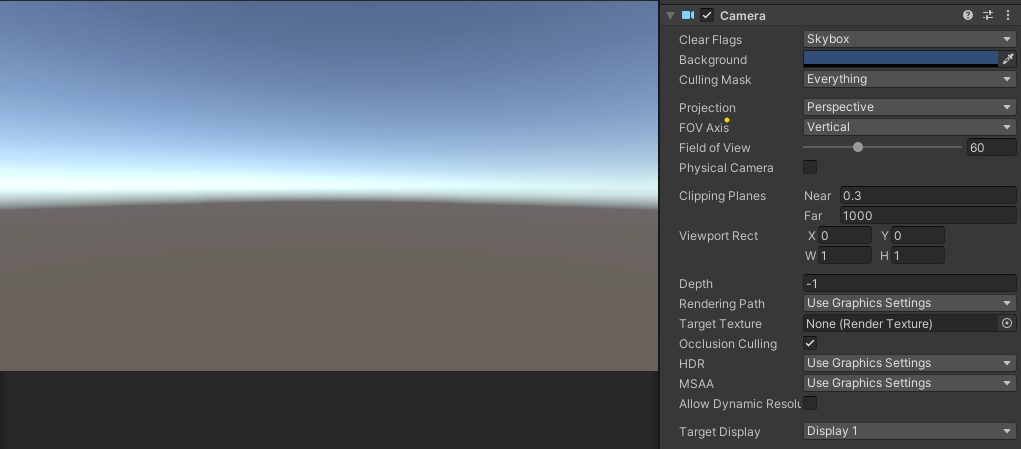
\includegraphics[width=\textwidth]{camera}
	\caption{Componente de cámara junto a su representación en pantalla.}
	\label{fig:camera}
\end{figure}

Una de las proyecciones que permite visualizar la escena lo más fiel a la realidad es la proyección en perspectiva cónica. Esta perspectiva es un sistema de representación gráfico basado en la proyección de un cuerpo tridimensional sobre un plano, auxiliándose en rectas proyectantes que pasan por un punto. Este sistema es el que más se asemeja a la visión humana, ya que se logra una aparente profundidad \cite{eduxg:perscon}, y es el empleado en Unity para la representación de objetos en la escena.

La forma en la que se aprovecha de cara a un videojuego de carreras es empleando la cámara en tercera persona, donde la cámara sigue al vehículo ligeramente alejada. Para un mayor realismo, se ha hecho uso de un sistema de cámaras dinámico ya programado más fluido llamado Cinemachine \cite{doc:cinemachine}. Este componente ha sido instalado desde propio Unity.

\subsection{Sistema de coordenadas}

El sistema de coordenadas engloba a toda la escena en la que nos hallamos. Esto provoca que las coordenadas de los \textit{GameObject} que se hallan en la jerarquía de objetos y que no tengan ningún otro por encima de ellos sean globales, es decir, que sean relativas a la escena en la que se halle el usuario. 

\begin{figure}[h]
	\centering
	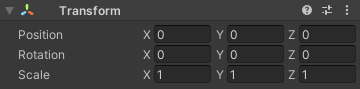
\includegraphics[width=\textwidth]{transform-coordenadas}
	\caption{Coordenadas en el \textit{Transform} de un objeto.}
	\label{fig:transform-coordenadas}
\end{figure}

En caso de que un \textit{GameObject} tenga un objeto padre en la jerarquía de objetos, su sistema de coordenadas será local en vez de global, lo que implica que su posición será relativa a la posición del objeto padre, esto es, dependerá de la jerarquía de objetos y no de la escena en sí.

Es importante tener en cuenta este concepto y su funcionamiento, ya que, aunque en apariencia es simple, puede provocar confusión a la hora de la colocación de un objeto, debido a que unas mismas coordenadas no generan el mismo posicionamiento en la escena con un objeto que depende de otro objeto (o de una jerarquía de objetos) que con un objeto que depende de la propia escena.

\subsection{Físicas}

Unity integra un sistema de físicas que permite a los \textit{GameObjects} tener un comportamiento físico convincente, donde deben poder tener una aceleración adecuada y verse afectados por las colisiones, la gravedad y otras fuerzas. Este sistema proporciona distintos componentes que manejan la simulación física, de manera que modificando los distintos ajustes se puede obtener objetos que se comporten pasivamente de una manera realista. Da la posibilidad de controlar estas físicas desde \textit{script}, por lo que se puede dotar a los objetos de un dinamismo muy diverso. En Unity, los conceptos principales de las físicas para los juegos en 2D y en 3D son iguales, pero la implementación es diferente, por lo que hay un motor específico para 2D y otro para 3D \cite{doc:physics}.

Los principales componentes en relación a las físicas son los \textit{Rigidbody} y los \textit{colliders} o colisionadores (estos últimos han sido explicados en el apartado de \textit{GameObject}). 

Un \textit{Rigidbody} es el componente principal que permite el comportamiento físico de un objeto. Al añadir este componente a un objeto, éste responderá de manera inmediata a la gravedad. Si, además, se añaden uno o más colisionadores al objeto, entonces éste será movido por las colisiones entrantes. La manera en la que ahora responderá el objeto ante el movimiento será mediante fuerzas aplicadas al mismo, y no mediante cambios directos en su transformada \cite{doc:rigidbody}.

También hay que tener en cuenta a los \textit{triggers}, los cuales no son componentes físicos como tal sino eventos que nos permiten modificar el comportamiento de un objeto y actúan dentro de los colisionadores. Estos eventos se activan indicando si un colisionador es un \textit{trigger} o no. A partir de esa activación, el colisionador deja de tener comportamiento físico y ahora puede ejercer las acciones que indique un componente mediante \textit{script}.

\subsection{Asset}

Los \textit{assets} o recursos son representaciones de cualquier ítem que pueda ser utilizado en el juego. Puede partir de un archivo creado de manera externa a Unity, como puede ser un modelo 3D, un archivo de audio, una imagen o cualquiera de los tipos de archivo que Unity soporta, así como aquellos que pueden ser creados dentro del mismo motor, como los controladores de animación o los mezcladores de audio \cite{doc:assets}.

En ``Fastastic Roads'' los \textit{assets} principales son los modelos de los vehículos y del escenario, los cuales son objetos 3D creados en Blender, acompañados de sus respectivas texturas.

\begin{figure}[h]
	\centering
	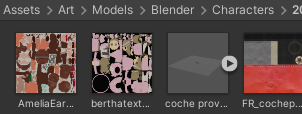
\includegraphics[width=\textwidth]{assets}
	\caption{Se pueden incluir todo tipo de \textit{assets} compatibles con Unity.}
	\label{fig:assets}
\end{figure}

\subsection{Prefab}

Los \textit{prefabs} u objetos prefabricados son \textit{GameObjects} a los cuales se les ha añadido distintos componentes y ajustado sus propiedades al valor adecuado al diseñador, de tal manera que se almacena como un conjunto para poder ser instanciado en adelante sin tener que integrar cada modelo individual con sus mismas propiedades, optimizando el tiempo de creación de objetos y pudiendo ser reutilizados tantas veces como se necesite, esto es, actuando como una plantilla a partir de la cual se pueden crear nuevas instancias del objeto en la escena \cite{doc:prefab}.

En el momento en el que un \textit{prefab} sea editado, se reflejará en todas las instancias producidas a partir de éste. No obstante, se pueden realizar modificaciones individuales para cada instancia.

\begin{figure}[h]
	\centering
	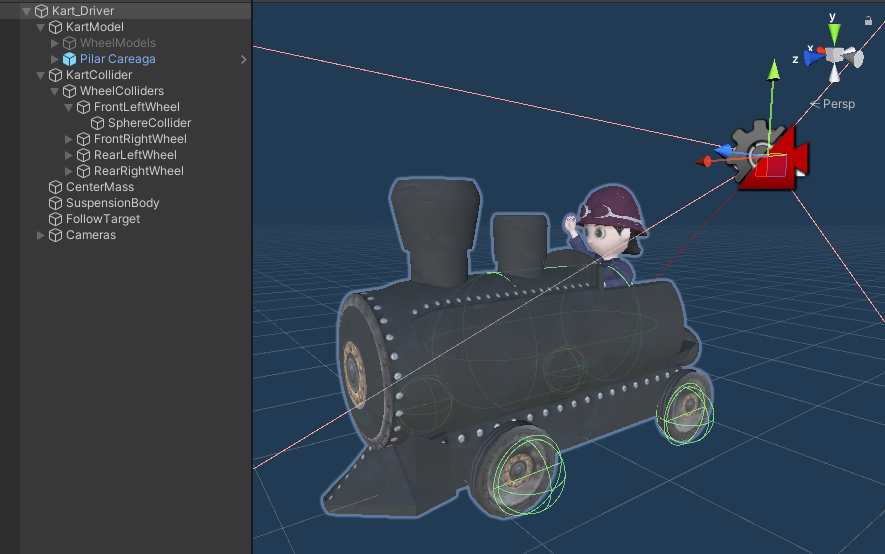
\includegraphics[width=\textwidth]{prefab-pilar}
	\caption{\textit{Prefab} del personaje de Pilar Careaga.}
	\label{fig:prefab-pilar}
\end{figure}

\subsection{Renderizado}

El renderizado 3D es el proceso de producción de una imagen basado en datos tridimensionales. Con el renderizado 3D, se convierten las mallas de modelos 3D (estas mallas se componen de vértices y caras triangulares que conectan estos vértices) en imágenes 2D \cite{doc:renderer}. 

Existen dos tipos principales:
\begin{itemize}
\tightlist
	\item Renderizado sin conexión (o prerrenderizado): el renderizado de fotogramas es suficientemente rápido como para que al renderizarse secuencialmente los diferentes fotogramas den la sensación de animación y movimiento de manera fluida.
	\item Renderizado en tiempo real: es el más común en videojuegos, donde el renderizado de fotogramas es suficientemente rápido como para que al renderizarse secuencialmente los diferentes fotogramas den la sensación de animación y movimiento de manera fluida. El objetivo es tratar de alcanzar una velocidad de renderizado mínima aceptable para el jugador, siendo 24 fotogramas/segundo el mínimo necesario para que el ojo humano pueda crear ``ilusión de movimiento''.
\end{itemize}

\subsection{Sistemas de entrada}

Los sistemas de entrada o \textit{inputs} permiten tener una interacción directa con los objetos del escenario a la hora de jugar. Unity soporta distintos dispositivos de entrada, entre ellos los convencionales como son el teclado, los \textit{joysticks}, \textit{joypads} y otros, así como pantallas táctiles, detección de movimiento de dispositivos móviles, micrófonos y cámaras web \cite{doc:input}.

Para poder moverse por el juego se requiere de un ratón para la selección de las opciones entre los menús y de un teclado o mando para manejar el vehículo en una partida.

\subsection{Sonido}

El sonido es un aspecto muy importante en un videojuego, pues es el encargado de transmitir las sensaciones auditivas respecto a las acciones que realiza el jugador o los elementos con los que interactúa, como puede ser accionar un botón, activar algún objeto, correr o el sonido de un motor entre otros, así como el sonido ambiente que engloba a una escena \cite{doc:sound}.

Unity provee al usuario de un sistema de sonido espacial 3D completo, así como de un sistema de mezcla y masterizado en tiempo real, jerarquías de mezcladores, instantáneas y efectos.

En el caso del juego, carece de sonido debido a las limitaciones temporales del proyecto. No obstante, es un objetivo a cumplir, proveyendo al juego de efectos de sonido y banda sonora.

\subsection{Multijugador}

El modo multijugador, bien sea en red local, red Internet o a pantalla partida (diversos jugadores en una misma pantalla), es un tipo de juego en el cual varios participantes compiten o colaboran en una partida de juego. Este es un modo muy atractivo para el usuario, ya que permite jugar e interactuar con más personas en el mismo juego.

Este modo, actualmente, no se encuentra disponible en el juego, pero, de nuevo, es una idea planteada con intención de ser integrada más adelante, pues hará más atractivas las partidas al tener más jugadores involucrados en ellas.

\section{Videojuegos de carreras} 

Mencionado con anterioridad, hay multitud de géneros en los videojuegos. Entre ellos se encuentran los videojuegos de conducción, donde, como su nombre indica, se tratan de juegos en los cuales se emula la conducción de un vehículo en un entorno virtual. 

Esta conducción puede ser muy similar a la real, factor principal de los videojuegos simuladores de conducción, o puede ser ``arcade'', cuyo término era originario de las primeras máquinas recreativas (o \textit{máquinas arcade}) y se utiliza también actualmente para designar un estilo de videojuegos que siguen los principios básicos que tenían esas máquinas, entre ellos el tener un diseño sencillo, controles fáciles de asimilar y dominar, niveles no muy extensos, con dificultad ascendente y con una escasa interrupción de juego entre niveles \cite{wikij:arcade}.

El entorno virtual puede representarse de diversas formas, como son los circuitos cerrados, donde se pueden realizar distintas pruebas como carreras competitivas o a contrarreloj y otra serie de pruebas como minijuegos (saltos de altura con el vehículo, superar obstáculos, etc.) u otras, o los escenarios de ``mundo abierto'', en los cuales se pueden realizar también estás pruebas pero con un elemento diferenciador, el cual es la libertad de conducción por el escenario sin interrupciones de ningún tipo en la partida.

Las carreras pueden ser muy diversas, pero los tipos principales generalmente son dos, que son las carreras competitivas, donde se cumple un determinado número de vueltas mientras se rivaliza contra varios contrincantes por llegar al primer puesto, y las carreras contrarreloj, donde la prioridad es realizar la vuelta más corta en tiempo al circuito, habiendo también un límite de vueltas a realizar.

En el caso de ``Fastastic Roads'', se trata de un videojuego de carreras arcade. Estas carreras son únicamente contrarreloj, pero el objetivo en adelante es añadir un modo de carreras competitivas en las que se puedan utilizar habilidades acordes a los vehículos que maneje el usuario. Por ello, las partidas se realizan en circuitos que son cerrados (no son abiertas, no hay posibilidad de moverse libremente fuera del escenario) y ha de cumplirse el número de vueltas requerido mientras un cronómetro de tiempo cuenta el tiempo que se tarda en dar una vuelta y un marcador indica el mejor tiempo realizado. Al acabar las vueltas indicadas, la partida finaliza devolviendo al usuario al menú hasta que se decida empezar una nueva.

\subsection{Puntos de control}

Los \textit{checkpoints} o puntos de control son posiciones del circuito, generalmente estratégicas y con un sentido dentro del juego (previo a bifurcaciones, caídas peligrosas y otros) indicadas previamente a elección del diseñador de juego. Estos puntos registran el cruce del jugador a través de ellos, de manera que permite realizar un conteo de vueltas legal, en el cual el jugador habrá pasado en un orden concreto sin posibilidad a realizar trampas de ningún tipo, y así obtener una vuelta válida.

Así mismo, en caso de que el vehículo se salga de la pista o vuelque, estos puntos de control permiten recolocar el vehículo del jugador en el último atravesado, para poder continuar la carrera de nuevo.